\paragraph*{Workload Vs Workflow} The term ``workflow'' is used in many
disciplines with different meaning. In the field of scientific computing,
``workflow'' assumes different meanings depending on the characteristics of the
computation, of the software tools used to support this computation, and of the
resources on which it is performed. Further, a workflow may indicate a whole
application, a description of the computational process of that application or,
more commonly, a series of tasks related by data dependences.

The lack of a consistent and shared definition of ``workflow'' hinders the
understanding of its properties and its relations with related concepts. For
example, we need to clarify the difference among ``workflow'', ``workload'',
``task'', or ``job'' but also between workflow template and instance, or
data-flow and control-flow. This is precondition to specify properly the design
of software systems that support the execution of scientific applications.

In this paper, we use the following definitions:

\begin{description}

  \item[Task.] A set of operations to be performed on a computing platform,
  alongside a description of the properties and dependences of those operations,
  and indications on how the dependences should be satisfied and the operations
  should be executed.

  \item[Job.] A unit of execution that performs one or more unit of work. Jobs
  relates to the resource on which they are executed. One or more tasks can be
  the units of work executed by a job.

  \item[Workload.] A set of tasks that can be executed concurrently, possibly
  related by a set of relations. For example, tasks of a workload can share one
  or more input files or communicate during execution.

  \item[Workflow.] Set of workloads, related by a set of relations that define
  the order in which each workload can be executed. Data dependences are the
  most common relations among workloads, used to define the precedence among
  their executions. Note that, formally, a workload can have a single task.

\end{description}

Each task may have an arbitrary number of properties like number of cores,
executables, or input/output files. Tasks may have precedence relations
depending on their data dependences or any other type of dependency mandated
by the application algorithms. Tasks with precedence relations have to be
executed serially, otherwise tasks can be executed concurrently. A workload is
defined as a set of tasks that can be executed concurrently. As such, a
workflow can be composed by a set of workloads.

The terms ``task'' and ``job'' are also used inconsistently across communities
that perform scientific computing. In this paper, ``job'' refers to the unit of
work that is submitted to a local resource management system (LRMS), like a
batch system or a scheduler. As such, a task can become a job when is scheduled
on a resource that exposes a LRMS but can also become a virtual machine or a
container when bootstrapped on an infrastructure supporting virtualization.
Tasks can be grouped into jobs, statically or dynamically, depending on the
resource capabilities and the task requirements.

Usually, workflows are represented as graphs in which tasks are vertices and
relations are edges~\cite{}. Often, graphs are supposed to be acyclic but graphs
with cycles have been used to represent workflows of workflows~\cite{}. In this
paper, a workflow template is a type of graph while a workflow instance is a
type of graph with a specific set of vertices and edges. Further, a graph is
``abstract'' when no resource properties are available for all vertices,
``concrete'' otherwise~\cite{}.

The distinction between an abstract and concrete graph highlights an important
element of the execution process of a workflow. Workflows can be specified
without indicating on what resources they should be executed. Accordingly, an
abstract graph can be interpreted as a formal description of the requirements
for the workflow execution. Once these requirements are matched by a set of
resource capabilities, the graph becomes concrete, i.e., a formal description
of the workflow execution process and its execution environment.

\subsection{ATLAS Workflow}

\begin{figure}
  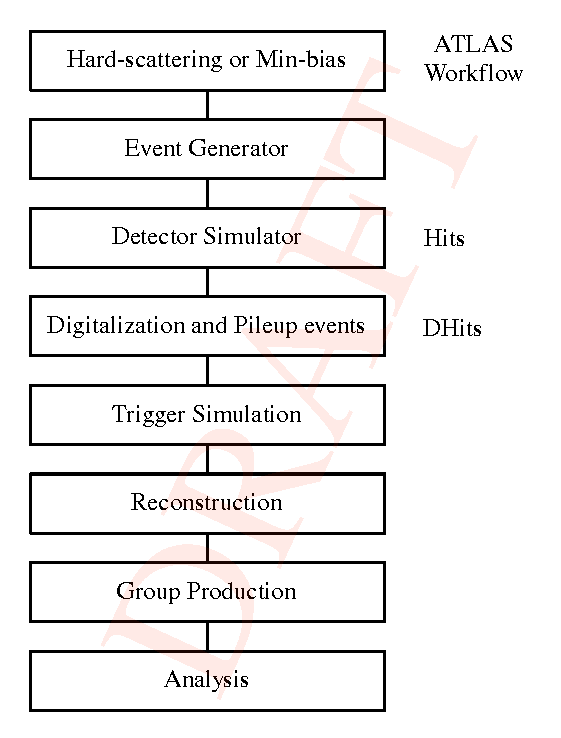
\includegraphics[width=\columnwidth]{figures/atlas_workflow.pdf}
  \caption{ATLAS Workflow}
\label{fig:atlas_workflow}
\end{figure}
